\section{Implementation}

Figure \ref{fig:Flowers} illustrates the transformations of a sketch to embroidery machine patterns in Sketch\&Stitch. 
Sketch\&Stitch's pipeline begins when the user calibrates her fabric and marker colors using a printable template and the system's mobile app. The user defines a color palette: a \textit{trace color} an optional \textit{insulation color} and up to six \textit{art colors}. Based on these colors, the system generates a color scheme for processing user input. The scheme is composed of the above \textit{trace, insulation} and \textit{art colors}, and three additional \textit{sticker colors}, for printing and recognizing Component and Embroidery Stickers, are selected from outside the user's palette.

\begin{figure} [t!]
\centering
  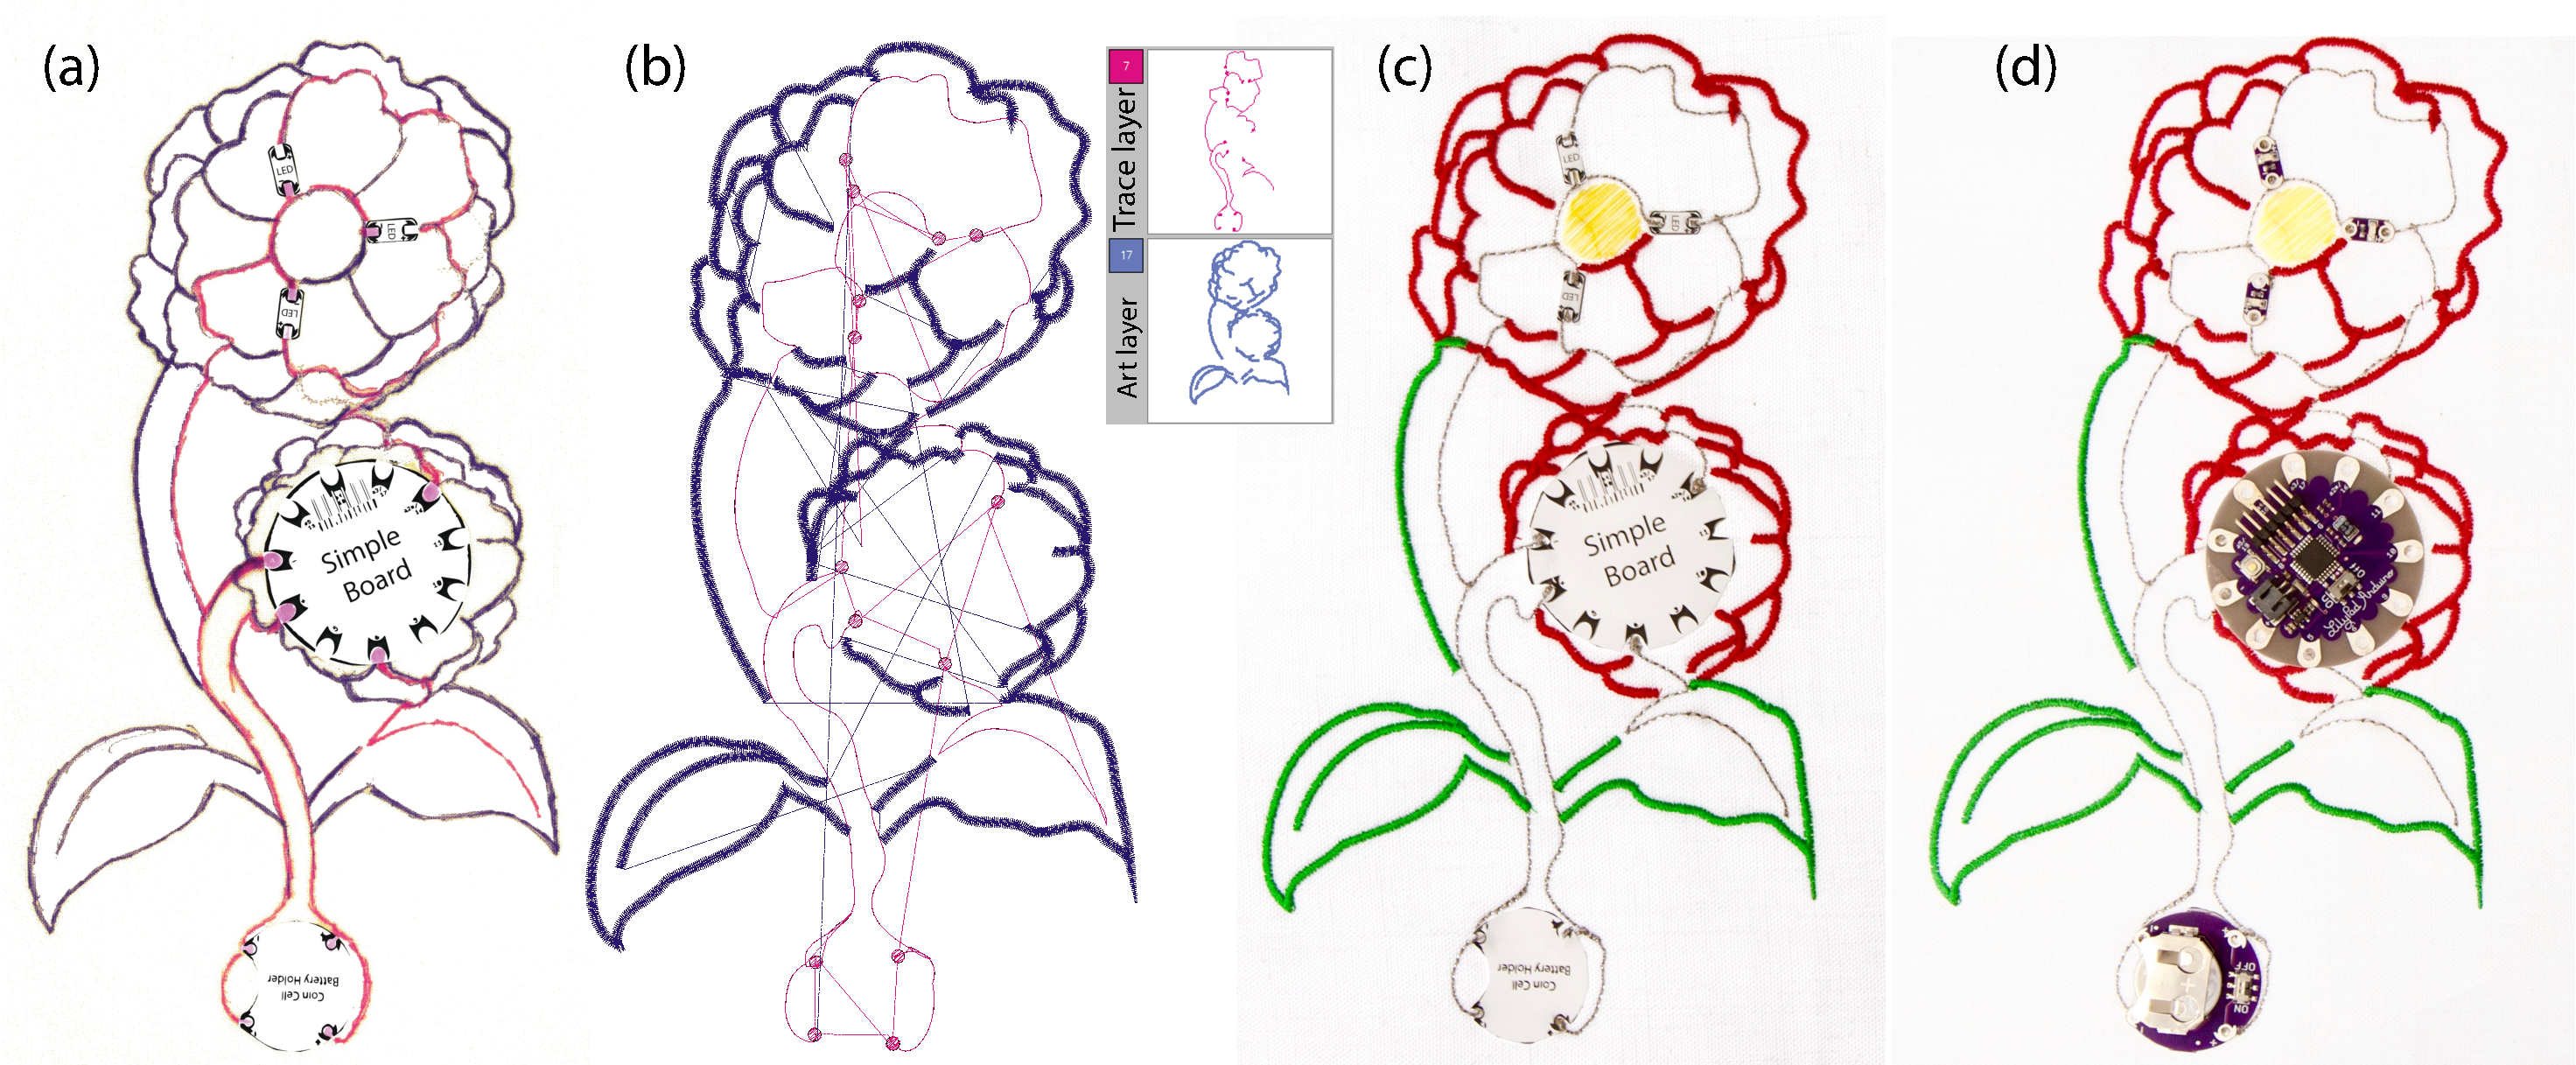
\includegraphics[width=1\columnwidth]{figures/Flowers}
  \caption{Sketch transformations: (a) localize and enhance captured sketch, (b) sketch separated into design layers based on a color scheme and tool path generated in embroidery software (the connecting lines signify the path between individual stitches), (c) embroidery finished, (d) final e-textile with stickers replaced by real components.}~\label{fig:Flowers}
  \vspace{-2.5em}
  \end{figure}

Every time the user is ready to embroider a sketch, she presses the capture button near the camera mount, and the mobile app snaps a picture of the hooped fabric and sketch. Below we describe the three following steps in Sketch\&Stitch pipeline. In our implementation we used OpenCV libraries for image processing and marker recognition. 

%The sketch is first localized in the image with help of visual markers on the hoop's frame, processed to reduce noise and enhance color, split into design layers based on a color scheme, fiducial Circuit Stickers are detected and replaced with appropriate patterns, design layers are sent to embroidery software to be digitized, and finally, digital embroidery patterns are sent to embroidery machine to be stitched. 


\subsection{Sketch Localization and Noise Reduction}
Once the sketch is captured, the system looks for a visual marker on the physical hoop to calculate its center and orientation, and applies the appropriate cropping mask to extract the sketch and store it at real-world scale.

The cropped image is then processed, adjusting contrast, reducing and merging redundant colors introduced during capturing, e.g., from changing pressure while sketching, and removing the fabric's background color (we discuss patterned base fabrics in Future Work).
%based on the system's color scheme

%The quality of embroidery depends highly on the quality of the captured image. Factors that affect the quality of an image include camera resolution, light setup and shadows, the flatness and texture of fabric, the quality of markers, and the amount of presser applied to makers while sketching. (we mention that is system design section)



\subsection{Color Filtering and Marker Detection}
Next, the system performs color filtering based on the established color scheme, to split the design into multiple design layers called the \emph{embroidery stack}. The stack is composed of a bottom layer, the trace layer, tinted with \textit{trace color}, and sequenced to be embroidered first with conductive thread; an insulation layer, tinted with \textit{insulation color}, and sequenced to be embroidered second with non-conductive thread; art layers, each tinted with an \textit{art color}; and finally the bridge layer, tinted with the third \textit{sticker color}, and scheduled to be embroidered last. The bridge layer contains bridge stitches that should be embroidered in conductive thread over exiting circuit traces without penetrating them.

To create the embroidery stack the system filters the sketch based on color scheme as follows: 
\begin{enumerate}
    \item Filter out Component Stickers' \textit{sticker colors}, e.g., black and white. This step removes the stickers from the sketch and leaves white space in their place.
    \item Filter for \textit{trace color}, e.g., red. This includes circuit traces, hand-sketched sensors, and the grid in \textit{sensor stickers}. All are stored in the trace layer.
    \item Filter for \textit{insulation color}, e.g., green. These objects are duplicated and stored in the trace layer and insulation layer.
    \item Filter for \textit{art colors}, storing each in a separate art layer.
    \item Filter for Embroidery Stickers' \textit{sticker color}, e.g., dark blue. Using the Harris corner detector in OpenCV, we detect the corners of each rectangle in Embroidery Stickers, and replace complete rectangles with the three shielding design layers described previously. These layers are merged with the trace layer, insulation layer, and bridge layer in the embroidery stack.
\end{enumerate}
 
%Based on the marker tip, we reduce the thickness of traces in order to force embroidery software to treat them as outlines, as opposed to closed shapes that need to be filled. This step avoids stitching thick conductive traces, which wastes a lot of thread and makes them more visible in the final design.


The system ignores all colors outside its scheme. If the user wants to enable incremental design, thread colors should also be outside the system's color scheme 
%(except for Component Sticker colors since they are ignored by the system) 
such that the system can differentiate sketched lines from already embroidered ones. 

\subsection{Stitch Mapping and Embroidering}
The embroidery stack is then sent to embroidery software. It converts objects in each layer into embroidery patterns. Based on the color of a layer, a pre-defined stitch type is used for it. Sketch\&Stitch then sends the resulting embroidery patterns to the embroidery machine. After checking these patterns on the machine's embedded display, the user threads the conductive thread first and starts embroidery, re-threading each time a new colored layer is ready to be stitched. All sketches and embroidery patterns are stored on the computer and can be accessed, modified, reused and shared from there.


%Our system matches stitch types to embroidery stack as follows: triple running stitch (2 mm length) for circuit traces and sensors, zigzag stitch (2.0 mm width, 0.3 mm spacing) for insulation, satin stitch (2.0 mm width, 0.5 mm spacing) for art pattern, and single running stitch (9 mm length) for bridge stitch. Embroidery software converts the stack into layers of embroidery patterns. The system send these patterns to an embroidery machine via a wireless connection. 





